\documentclass[12pt,letterpaper,titlepage]{article}
\usepackage{fontspec}
\defaultfontfeatures{Mapping=tex-text}
\usepackage{xunicode}
\usepackage{xltxtra}
%\setmainfont{???}
\usepackage{amsmath}
\usepackage{amsfonts}
\usepackage{amssymb}
\setcounter{secnumdepth}{0}
\setmainfont{Times New Roman}
\showboxdepth=\maxdimen
\showboxbreadth=\maxdimen

\usepackage[tocflat]{tocstyle}
\usetocstyle{allwithdot}
\usepackage[bottom]{footmisc}

\usepackage{karnaugh-map}
\usepackage{paracol}
\usepackage{wrapfig}
\globalcounter{table}
\globalcounter{figure}
\usepackage{graphicx}
\usepackage[left=1in,right=1in,top=1in,bottom=1in]{geometry}
\graphicspath{{img/}}
\author{Jacob Abel}
\title{Project 1}
\usepackage{ifthen}
\usepackage{xcolor}
\usepackage{tikz}
\usetikzlibrary{calc}
\setlength{\parskip}{0.5em}

\pgfkeys{
  /sevenseg/.is family, /sevenseg,
  slant/.estore in      = \sevensegSlant,     % vertical slant in degrees
  size/.estore in       = \sevensegSize,      % length of a segment
  shrink/.estore in     = \sevensegShrink,    % avoids overlapping of segments
  line width/.estore in = \sevensegLinewidth, % thickness of the segments
  line cap/.estore in   = \sevensegLinecap,   % end cap style rect, round, butt
  oncolor/.estore in    = \sevensegOncolor,   % color of an ON segment
  offcolor/.estore in   = \sevensegOffcolor,  % color of an OFF segment
}

\pgfkeys{
  /sevenseg,
  default/.style = {slant = 0, size = 1em, shrink = 0.1,
                    line width = 0.15em, line cap = butt,
                    oncolor = red, offcolor = gray}
}

%===============================================
%                     a b c d e f g - segment values
% \sevenseg[options]{{1,1,1,1,1,1,0,}}
%
\newcommand{\sevenseg}[2][]% options values
{%
\pgfkeys{/sevenseg, default, #1}%
\def\sevensegarray{#2}%
  \begin{tikzpicture}%
    % first define the position of the 6 corner points
    \path (0,0) ++(0,0)                             coordinate (P1);
    \path (0,0) ++(\sevensegSize,0)                 coordinate (P2);
    \path (0,0) ++(90-\sevensegSlant:\sevensegSize) coordinate (P3);
    \path (P2)  ++(90-\sevensegSlant:\sevensegSize) coordinate (P4);
    \path (P3)  ++(90-\sevensegSlant:\sevensegSize) coordinate (P5);
    \path (P4)  ++(90-\sevensegSlant:\sevensegSize) coordinate (P6);
    % then step through the 1/0 values in the segment array
    \foreach \i in {0,...,6}%
    {
      \pgfmathparse{\sevensegarray[\i]}
      \ifthenelse{\equal{\pgfmathresult}{1}}%
        {\let\mycolor=\sevensegOncolor}%  segment is on
        {\let\mycolor=\sevensegOffcolor}% segment is off
      \tikzstyle{segstyle} = [draw=\mycolor, line width = \sevensegLinewidth,
                              line cap = \sevensegLinecap]
      %-----------------------
      \ifthenelse{\equal{\i}{0}}{\path[segstyle]
        (${1-\sevensegShrink}*(P5)+\sevensegShrink*(P6)$)
        -- ($\sevensegShrink*(P5)+{1-\sevensegShrink}*(P6)$);}{} % a
      \ifthenelse{\equal{\i}{1}}{\path[segstyle]
        (${1-\sevensegShrink}*(P6)+\sevensegShrink*(P4)$)
        -- ($\sevensegShrink*(P6)+{1-\sevensegShrink}*(P4)$);}{} % b
      \ifthenelse{\equal{\i}{2}}{\path[segstyle]
        (${1-\sevensegShrink}*(P4)+\sevensegShrink*(P2)$)
        -- ($\sevensegShrink*(P4)+{1-\sevensegShrink}*(P2)$);}{} % c
      \ifthenelse{\equal{\i}{3}}{\path[segstyle]
        (${1-\sevensegShrink}*(P1)+\sevensegShrink*(P2)$)
        -- ($\sevensegShrink*(P1)+{1-\sevensegShrink}*(P2)$);}{} % d
      \ifthenelse{\equal{\i}{4}}{\path[segstyle]
        (${1-\sevensegShrink}*(P1)+\sevensegShrink*(P3)$)
        -- ($\sevensegShrink*(P1)+{1-\sevensegShrink}*(P3)$);}{} % e
      \ifthenelse{\equal{\i}{5}}{\path[segstyle]
        (${1-\sevensegShrink}*(P3)+\sevensegShrink*(P5)$)
        -- ($\sevensegShrink*(P3)+{1-\sevensegShrink}*(P5)$);}{} % f
      \ifthenelse{\equal{\i}{6}}{\path[segstyle]
        (${1-\sevensegShrink}*(P3)+\sevensegShrink*(P4)$)
        -- ($\sevensegShrink*(P3)+{1-\sevensegShrink}*(P4)$);}{} % g
    }
  \end{tikzpicture}%
}

\newcommand{\sevensegnum}[2][]% sample characvters
{%
  \ifthenelse{\equal{#2}{0}}{\sevenseg[#1]{{1,1,1,1,1,1,0,}}}{%
  \ifthenelse{\equal{#2}{1}}{\sevenseg[#1]{{0,1,1,0,0,0,0,}}}{%
  \ifthenelse{\equal{#2}{2}}{\sevenseg[#1]{{1,1,0,1,1,0,1,}}}{%
  \ifthenelse{\equal{#2}{3}}{\sevenseg[#1]{{1,1,1,1,0,0,1,}}}{%
  \ifthenelse{\equal{#2}{4}}{\sevenseg[#1]{{0,1,1,0,0,1,1,}}}{%
  \ifthenelse{\equal{#2}{5}}{\sevenseg[#1]{{1,0,1,1,0,1,1,}}}{%
  \ifthenelse{\equal{#2}{6}}{\sevenseg[#1]{{1,0,1,1,1,1,1,}}}{%
  \ifthenelse{\equal{#2}{7}}{\sevenseg[#1]{{1,1,1,0,0,0,0,}}}{%
  \ifthenelse{\equal{#2}{8}}{\sevenseg[#1]{{1,1,1,1,1,1,1,}}}{%
  \ifthenelse{\equal{#2}{9}}{\sevenseg[#1]{{1,1,1,1,0,1,1,}}}{%
  \ifthenelse{\equal{#2}{A}}{\sevenseg[#1]{{1,1,1,0,1,1,1,}}}{%
  \ifthenelse{\equal{#2}{B}}{\sevenseg[#1]{{0,0,1,1,1,1,1,}}}{%
  \ifthenelse{\equal{#2}{C}}{\sevenseg[#1]{{0,0,0,1,1,0,1,}}}{%
  \ifthenelse{\equal{#2}{D}}{\sevenseg[#1]{{0,1,1,1,1,0,1,}}}{%
  \ifthenelse{\equal{#2}{E}}{\sevenseg[#1]{{1,0,0,1,1,1,1,}}}{%
  \ifthenelse{\equal{#2}{F}}{\sevenseg[#1]{{1,0,0,0,1,1,1,}}}{%
  {\sevenseg[#1]{{0,0,0,0,0,0,0,}}}}}}}}}}}}}}}}}}}%
}

\begin{document}
\maketitle


\tableofcontents
\pagebreak
\listoftables

\listoffigures

\pagebreak
\begin{raggedright}

\section{Purpose}

\begin{wrapfigure}[13]{R}{0.4\textwidth}
\centering
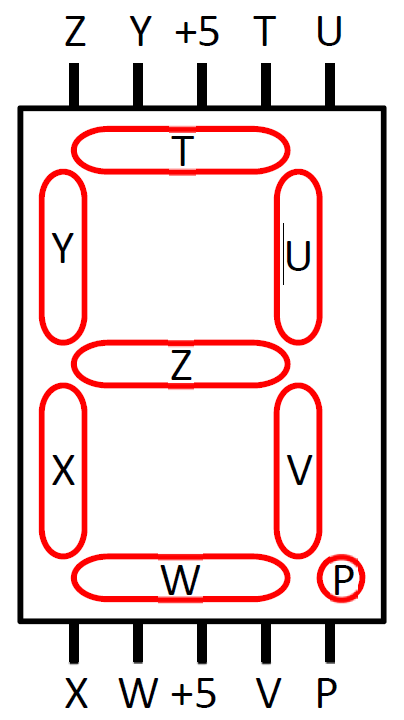
\includegraphics[width=2.75cm]{led}
\caption[7-Segment Display Pinout]{\raggedright 7-Segment Display Pinout sourced from the ECE2504 Lab Manual}
\end{wrapfigure}
The purpose of this circuit was to design, optimise, simulate, and construct a basic combinational circuit. This required basic wiring skills, application of combinational logic design skills, and usage of logic modelling, simulation, and hardware programmer software.

\section{Problem Specification}

\begin{wraptable}[12]{R}{0.6\textwidth}
\label{decto6412}
\centering
\begin{tabular}{|c|c|c|c|c|c|}\hline
Decimal & 0    & 1    & 2    & 3    & 4    \\\hline
641-2   & 0000 & 0010 & 0101 & 0111 & 0100 \\\hline
\end{tabular}
\begin{tabular}{|c|c|c|c|c|c|}\hline
Decimal & 5    & 6    & 7    & 8    & 9    \\\hline
641-2   & 0110 & 1000 & 1010 & 1101 & 1111 \\\hline
\end{tabular}
\caption[1-digit decimals to 4-bit 641-2 codes]{\raggedright 1-digit decimals to 4-bit 641-2 codes sourced from the Project 1 Specifications}
\bigskip

\label{7seg}
\begin{tabular}{|c|c|c|c|c|} \hline
0&1&2&3&4\\
 \sevensegnum[size = 2em, line cap = butt, oncolor=red]{0}
&\sevensegnum[size = 2em, line cap = butt, oncolor=red]{1}
&\sevensegnum[size = 2em, line cap = butt, oncolor=red]{2}
&\sevensegnum[size = 2em, line cap = butt, oncolor=red]{3}
&\sevensegnum[size = 2em, line cap = butt, oncolor=red]{4}\\
0000001 & 1001111 & 0010010 & 0000110 & 1001100\\\hline
5&6&7&8&9\\
 \sevensegnum[size = 2em, line cap = butt, oncolor=red]{5}
&\sevensegnum[size = 2em, line cap = butt, oncolor=red]{6}
&\sevensegnum[size = 2em, line cap = butt, oncolor=red]{7}
&\sevensegnum[size = 2em, line cap = butt, oncolor=red]{8}
&\sevensegnum[size = 2em, line cap = butt, oncolor=red]{9}\\
0100100 & 0100000 & 0001111 & 0000000 & 0001000\\\hline
\end{tabular}
\caption[7-segment display configurations]{\raggedright 7-segment display configurations (TUVWXYZ) sourced from the Project 1 Specifications}
\end{wraptable}

This project requires that the final circuit convert a 641-2 (4-bit negatively weighted decimal) code into a 7-bit code for a 7-segment display with each lit part of the display corresponding to a 0-value bit. The circuit could be designed with only 2-input NAND gates and inverters. The required software for the modelling and simulation of the circuit was Quartus.

Final deliverables include a circuit diagram of the completed circuit, a Quartus project archive of the latest revision of the circuit project, and this technical report detailing the project specifications as well as the development history and design process. Table 1 and Table 2 detail the mapping of decimal digits onto both the 641-2 codes as well as the 7-segment display codes. Figure 1 shows the pin mapping for the 7-Segment display.


\pagebreak
\section{Design Process}


\begin{wraptable}[24]{R}{0.6\textwidth}
\centering
\begin{tabular}{|c||c|c|c|c||c|c|c|c|c|c|c|}\hline
$Dec$ & $A$ & $B$ & $C$ & $D$ & T & U & V & W & X & Y & Z\\\hline\hline
0         & 0   & 0   & 0   & 0   & 0 & 0 & 0 & 0 & 0 & 0 & 1\\\hline
N/A       & 0   & 0   & 0   & 1   & - & - & - & - & - & - & -\\\hline
1         & 0   & 0   & 1   & 0   & 1 & 0 & 0 & 1 & 1 & 1 & 1\\\hline
N/A       & 0   & 0   & 1   & 1   & - & - & - & - & - & - & -\\\hline
4         & 0   & 1   & 0   & 0   & 1 & 0 & 0 & 1 & 1 & 0 & 0\\\hline
2         & 0   & 1   & 0   & 1   & 0 & 0 & 1 & 0 & 0 & 1 & 0\\\hline
5         & 0   & 1   & 1   & 0   & 0 & 1 & 0 & 0 & 1 & 0 & 0\\\hline
3         & 0   & 1   & 1   & 1   & 0 & 0 & 0 & 0 & 1 & 1 & 0\\\hline
6         & 1   & 0   & 0   & 0   & 0 & 1 & 0 & 0 & 0 & 0 & 0\\\hline
N/A       & 1   & 0   & 0   & 1   & - & - & - & - & - & - & -\\\hline
7         & 1   & 0   & 1   & 0   & 0 & 0 & 0 & 1 & 1 & 1 & 1\\\hline
N/A       & 1   & 0   & 1   & 1   & - & - & - & - & - & - & -\\\hline
N/A       & 1   & 1   & 0   & 0   & - & - & - & - & - & - & -\\\hline
8         & 1   & 1   & 0   & 1   & 0 & 0 & 0 & 0 & 0 & 0 & 0\\\hline
N/A       & 1   & 1   & 1   & 0   & - & - & - & - & - & - & -\\\hline
9         & 1   & 1   & 1   & 1   & 0 & 0 & 0 & 1 & 1 & 0 & 0\\\hline
\end{tabular}
\caption{7 Segment Display Truth Table}
\end{wraptable}
The first stage of the design process was to identify all necessary input and output variables. The 4-bit input 641-2 code was split into variables A, B, C, and D with A representing the most significant bit. The 7-Segment display bits were assigned to bits T, U, V, W, X, Y, and Z. When grouping the 7-Segment display bits together, T is always the first bit.

Immediately following this step, the truth table was laid out. One assumption with this truth table was that non legal 641-2 codes were considered invalid. This resulted in Table 3. Following the completion of the truth table, a K-Map was prepared for each output variable. Figure 2 through figure 8 in Appendix A are the corresponding K-maps for output variables T-Z. With the K-map groupings, it was decided that Sum of Products groupings would be used as Product of Sums groupings tend to take more NAND gates to implement. However, if the project was to be done again with solely NOR gates, Product of Sums would be used.

After the K-maps were grouped the equations for the outputs were derived from the groupings and stored in Table 4. Additionally, common terms were identified and marked in this table.

\begin{table}[ht]
\centering
\begin{tabular}{|c|l|c|c|c|c|c|}\hline
Output & Sum of Products & $(A'D)$ & $(C'D')$ & $(BC'D')$ & $(B'C)$ & $(BD')$ \\\hline
T & $A'B'C+BC'D'$  & 0 & 1 & 1 & 1 & 0 \\\hline
U & $AC'D'+BCD'$   & 0 & 1 & 0 & 0 & 0 \\\hline
V & $A'C'D$        & 1 & 0 & 0 & 0 & 0 \\\hline
W & $AC+B'C+BC'D'$ & 0 & 1 & 1 & 1 & 1 \\\hline
X & $BD'+C$        & 0 & 0 & 0 & 0 & 1 \\\hline
Y & $A'D+B'C$      & 1 & 0 & 0 & 1 & 0 \\\hline
Z & $A'B'+B'C$     & 0 & 0 & 0 & 1 & 0 \\\hline
\end{tabular}
\caption{Circuit Instances}
\end{table}

\newpage
\begin{wraptable}[15]{R}{0.6\textwidth}
\centering
\def\arraystretch{1.5}
\begin{tabular}{|c|l|}\hline
Variable & Optimised Equation \\\hline
I  & $A'D$                  \\\hline
J  & $C'D'$                 \\\hline
K  & $B'C$                  \\\hline
L  & $(BJ)'$                \\\hline
M  & $BD'$                  \\\hline
T  & $A'K+L'$               \\\hline
U  & $AJ+CM$                \\\hline
V  & $C'I$                  \\\hline
W  & $AC+K+L'$              \\\hline
X  & $M+C$                  \\\hline
Y  & $I+K$                  \\\hline
Z  & $A'B'+K$               \\\hline
\end{tabular}
\caption{Optimised Circuit}
\end{wraptable}

Following identification of common terms, all common terms were pulled out of the equations and substituted with variables I through M. These variables as seen in Table 5 exist to simplify the equations and reduce the quantity of gates in use. 9 AND gates and 11 inverters were removed from the circuit. Compared to the optimised circuit with 11 AND gates, 7 OR gates, and 9 Inverters, this results in a 45\% decrease in AND gates and a 55\% decrease in Inverters. The optimised circuit is still 100\% functionally equivalent to the original version.

\bigskip\bigskip
\bigskip\bigskip

\section{Implementation}
\begin{wraptable}[18]{r}{0.6\textwidth}
\centering
\begin{tabular}{|c||c|c|}\hline
$Dec$ & ABCD & TUVWXYZ\\\hline\hline
0         & 0000 & 0000001\\\hline
1         & 0010 & 1001111\\\hline
2         & 0101 & 0010010\\\hline
3         & 0111 & 0000110\\\hline
4         & 0100 & 1001100\\\hline
5         & 0110 & 0100100\\\hline
6         & 1000 & 0100000\\\hline
7         & 1010 & 0001111\\\hline
8         & 1101 & 0000000\\\hline
9         & 1111 & 0001100\\\hline
\end{tabular}
\caption{Simulation Results}
\end{wraptable}

At this point, the circuit was implemented in Quartus. The final circuit diagram is provided in Appendix B. The final design was then simulated with the results displayed in Table 6. The raw waveform of the simulation is provided in Appendix C. As shown in the table the results are identical to the legal values in Table 3. 

Once simulation proved that the circuit was valid in theory, it was programmed onto the DE-0 FPGA development board and the board was wired into an LED with a pinout listed in Table 7 in Appendix D. The 4 dip switches on the board toggled the values of ABCD with DIP3 corresponding to A.



\section{Validation}
Final validation of the completed circuit was to cycle through all legal values manually on the FPGA board using the dip switches and the LED 7-Segment display. During this process there were no issues and the circuit worked properly.


\section{Conclusion}
This project was a worthwhile exercise that demonstrated knowledge in basic combinational circuit design and technical documentation. The requirements were sufficiently outlined and documented. 

Given time to repeat the project, greater investment could be placed in optimising as alternative gate arrangements may have been able to result in a smaller total gate cost or shorter propagation delay. Otherwise, this implementation can be considered a complete success.

\pagebreak

\section{Appendix A: Karnaugh Maps}
\begin{paracol}{3}
\begin{figure}[h]
\centering
\resizebox{5cm}{!} {
\begin{karnaugh-map}[4][4][1][$CD$][$AB$]
  \minterms{2,4}
  \indeterminants{1,3,9,11,12,14}
  \autoterms[0]
  \implicant{3}{2}
  \implicant{4}{12}
\end{karnaugh-map}}
\vspace{-1cm}
\caption{Output T K-Map}
\end{figure}

\switchcolumn
\begin{figure}[h]
\centering
\resizebox{5cm}{!} {
\begin{karnaugh-map}[4][4][1][$CD$][$AB$]
  \minterms{6,8}
  \indeterminants{1,3,9,11,12,14}
  \autoterms[0]
  \implicant{6}{14}
  \implicant{12}{8}
\end{karnaugh-map}}
\vspace{-1cm}
\caption{Output U K-Map}
\end{figure}

\switchcolumn
\begin{figure}[h]
\centering
\resizebox{5cm}{!} {
\begin{karnaugh-map}[4][4][1][$CD$][$AB$]
  \minterms{5}
  \indeterminants{1,3,9,11,12,14}
  \autoterms[0]
  \implicant{1}{5}
\end{karnaugh-map}}
\vspace{-1cm}
\caption{Output V K-Map}
\end{figure}

\switchcolumn
\begin{figure}[h]
\centering
\resizebox{5cm}{!} {
\begin{karnaugh-map}[4][4][1][$CD$][$AB$]
  \minterms{2,4,10,15}
  \indeterminants{1,3,9,11,12,14}
  \autoterms[0]
  \implicant{15}{10}
  \implicantedge{3}{2}{11}{10}
  \implicant{4}{12}
\end{karnaugh-map}}
\vspace{-1cm}
\caption{Output W K-Map}
\end{figure}
\switchcolumn

\begin{figure}[h]
\centering
\resizebox{5cm}{!} {
\begin{karnaugh-map}[4][4][1][$CD$][$AB$]
  \maxterms{0,5,8,13}
  \indeterminants{1,3,9,11,12,14}
  \autoterms[1]
  \implicant{3}{10}
  \implicantedge{4}{12}{6}{14}
\end{karnaugh-map}}
\vspace{-1cm}
\caption{Output X K-Map}
\end{figure}
\switchcolumn

\begin{figure}[h]
\centering
\resizebox{5cm}{!} {
\begin{karnaugh-map}[4][4][1][$CD$][$AB$]
  \minterms{2,5,7,10}
  \indeterminants{1,3,9,11,12,14}
  \autoterms[0]
  \implicant{1}{7}
  \implicantedge{3}{2}{11}{10}
\end{karnaugh-map}}
\vspace{-1cm}
\caption{Output Y K-Map}
\end{figure}
\switchcolumn\switchcolumn
\begin{figure}[h]
\centering
\resizebox{5cm}{!} {
\begin{karnaugh-map}[4][4][1][$CD$][$AB$]
  \minterms{0,2,10}
  \indeterminants{1,3,9,11,12,14}
  \autoterms[0]
  \implicant{0}{2}
  \implicantedge{3}{2}{11}{10}
\end{karnaugh-map}}
\vspace{-1cm}
\caption{Output Z K-Map}
\end{figure}
\end{paracol}
\pagebreak

\section{Appendix B: 641-2 To 7-Segment Circuit Diagram}
\begin{center}
\includegraphics[width=0.75\textwidth]{circuit}
\end{center}
\clearpage

\section{Appendix C: Simulation Waveform}
\begin{center}
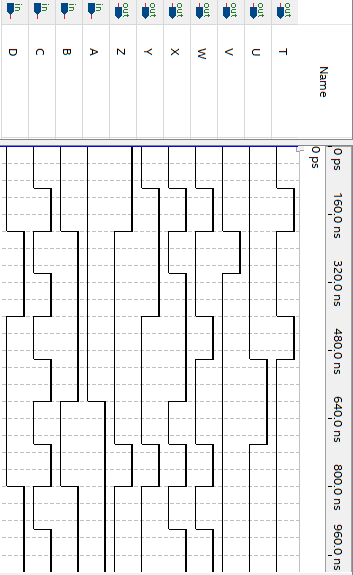
\includegraphics[width=0.75\textwidth]{wave}
\end{center}
\clearpage

\section{Appendix D: Pinouts and Wiring Charts}

\vspace{5cm}

\begin{paracol}{2}
\centering
\begin{table}[ht]
\centering
\def\arraystretch{1.5}
\begin{tabular}{|c|l|}\hline 
LED Pin & DE-0 GPIO Pin \\\hline 
T & GPIO\_16 (9) \\\hline 
U & GPIO\_14 (7) \\\hline 
V & GPIO\_128 (35) \\\hline 
W & GPIO\_130 (37) \\\hline 
X & GPIO\_132 (39) \\\hline 
Y &  GPIO\_18 (13) \\\hline 
Z & GPIO\_110 (15) \\\hline 
P & Do not connect. \\\hline 
+5V Top & VCC\_SYS (11) \\\hline 
+5V Bottom & Do not connect. \\\hline 
\end{tabular} 
\caption[LED Wiring Chart]{LED Wiring Chart sourced from the Project 1 Specifications}
\end{table}
\switchcolumn
\centering
\begin{table}[ht]
\centering
\def\arraystretch{1.5}
\begin{tabular}{|c|c|}\hline 
Variable & Dip Switch \\\hline 
A & DIP3 \\\hline  
B & DIP2 \\\hline  
C & DIP1 \\\hline  
D & DIP0 \\\hline 
  &      \\\hline 
  &      \\\hline 
  &      \\\hline 
  &      \\\hline 
  &      \\\hline 
  &      \\\hline 
\end{tabular} 
\caption{DIP Switch Pinout}
\end{table}
\end{paracol}
\end{raggedright}
\end{document}
